\documentclass[tikz,border=6pt]{standalone}
% Shared style for the HERMESS schematic figures (compiled by build.sh).
% ETH palette; Latin Modern (the LaTeX default) to match the documentation.
\usepackage{amsmath}
\usepackage{tikz}
\usetikzlibrary{arrows.meta,positioning,calc,shapes.geometric,circuits.ee.IEC}
\definecolor{ethblue}{HTML}{215CAF}
\definecolor{ethpetrol}{HTML}{007894}
\definecolor{ethgrey}{HTML}{6F6F6F}
\tikzset{
  block/.style      = {draw=ethblue, thick, fill=ethblue!8, minimum height=9mm,
                       minimum width=16mm, inner sep=2.5pt, align=center},
  sum/.style        = {draw=ethblue, thick, circle, fill=white, minimum size=4.5mm, inner sep=0pt},
  sig/.style        = {-{Latex[length=2.4mm]}, thick},
  wire/.style       = {thick},
  node distance     = 9mm and 12mm,
  every node/.style = {font=\small},
  lbl/.style        = {font=\small, inner sep=1.5pt},
  port/.style       = {font=\small\itshape, text=ethgrey},
}

\begin{document}
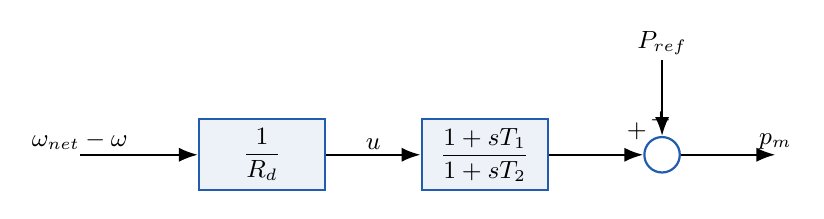
\begin{tikzpicture}
  \node[block] (droop) {$\dfrac{1}{R_d}$};
  \node[block, right=12mm of droop] (ll) {$\dfrac{1 + sT_1}{1 + sT_2}$};
  \node[sum, right=12mm of ll] (s) {};
  \node[lbl] at ($(s)+(-0.32,0.30)$) {$+$};
  \node[lbl] at ($(s)+(-0.02,0.44)$) {$+$};
  \draw[sig] ($(droop.west)+(-1.5,0)$) node[above, lbl] {$\omega_{net} - \omega$} -- (droop);
  \draw[sig] (droop) -- (ll) node[midway, above, lbl] {$u$};
  \draw[sig] (ll) -- (s);
  \draw[sig] ($(s)+(0,1.2)$) node[above, lbl] {$P_{ref}$} -- (s);
  \draw[sig] (s.east) -- ++(1.2,0) node[above, lbl] {$p_m$};
\end{tikzpicture}
\end{document}
